\documentclass[a4paper]{article}
\setlength\parindent{0pt}
\usepackage[top=1.5in,bottom=1.5in,left=1.5in,right=1.5in]{geometry}
\usepackage{graphicx}
\usepackage{amssymb}
\usepackage{amsmath}
\usepackage{mdwlist}
\usepackage{changepage}
\usepackage{tikz}
\begin{document}


\textsc{Building the Tree} \\

11$^\circ$ We have our sequences, our evolutionary distances, and a metric that corresponds to a phylogenetic tree. How do we actually get our phylogenetic tree? We turn to the \emph{Cherry-Picking Theorem} and the \emph{Neighbor-Joining Algorithm} for the answer. These algorithms are given without too much explanation at this point. Essentially, one begins with a `template tree' or network, then using the above information, one decides whether or not the nodes in the template tree belong or should be `pruned'. This process results in a phylogenetic tree $T$ using our metric $d_T$. \\

\begin{adjustwidth}{.5in}{0pt}
\textbf{Theorem 2 (Computational Cherry-Picking Theorem).} Let $d$ be a tree metric on $[n]$. For every pair $i,j \in [n]$ set
\[ Q_d(i,j) = (n-2) \cdot d(i,j) - \sum_{k \neq i} d(i,k) - \sum_{k \neq j} d(j,k). \] 
Then the pair $x,y \in [n]$ that minimizes $Q_d(x,y)$ is a cherry in the tree. \\ 
\end{adjustwidth}

The above theorem is a computationally superior form of a more theoretically relevant statement of the Cherry-Picking Theorem. Now that we know how to pick  a cherry out of a tree, we use the Neighbor-Joining Algorithm to build our tree. \\

\newpage

\begin{adjustwidth}{.5in}{0pt}
\textbf{Algorithm 3 (Neighbor-joining algorithm).} \\
Input: A dissimilarity map $d$ on the set $[n]$. \\
Output: A phylogenetic tree $T$ whose tree metric $d_T$ is ``close'' to $d$. \\

\emph{Step 1:} Construct the $n \times n$ matrix $Q_d$ whose $(i,j)$-entry is given by Theorem 2, and identify the minimum off-diagonal entry $Q_d(x,y)$. \\

\emph{Step 2:} Remove $x,y$ from the tree, thereby creating a new leaf $z$. For each leaf $k$ among the remaining $n - 2$ leaves, set
\[ d(z,k) = \frac{1}{2}(d(x,k) + d(y,k) - d(x,y)). \]

This replaces the $n \times n$ matrix $Q_d$ by an $(n -1) \times (n-1)$ matrix. Return to Step 1 until there are no more leaves to collapse. \\

\emph{Step 3}: Output the tree $T$. The edge lengths of $T$ are determined recursively: if $(x,y)$ is a cherry connected to node $z$ as in Step 2, then the edge from $x$ to $z$ has length $d(x,k) - d_T(z,k)$ and the edge from $y$ to $z$ has length $d(y,k) - d_T(z,k)$. \\
\end{adjustwidth}

Using the Cherry-Picking Theorem and the Neighbor-Joining Algorithm on our metric, we receive the following phylogenetic tree: \\
\begin{center}
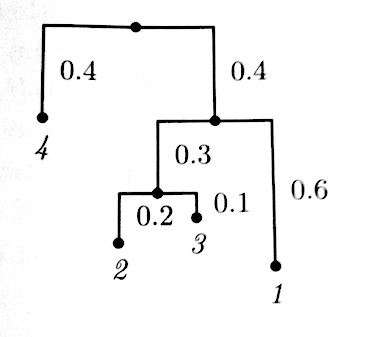
\includegraphics[width=200px]{photo.JPG}
\end{center}

\bigskip
\centerline{
\tikzpicture[thick,scale=1.8]
\tikzstyle{every node}=[draw,shape=circle,fill=blue!15];
\path (0,0) node (a) {\textsc{root}};
\path (-1.6,.4) node (b) {hi};
\path (1.6,.4) node (c) {hi};
\path (2.0,.7) node (d) {hi};
\path (-2.2,.9) node (e) {hi};
\path (-1.2,.8) node (f) {hi};
\path (0,1) node (g) {hi};
\draw (a) -- (b)
      (a) -- (c)
      (c) -- (d)
      (c) -- (g)
      (d) -- (e)
      (d) -- (f);
\endtikzpicture
}
\bigskip\smallskip
\centerline{Figure 5: Tree/Form}

\end{document}
